% Archivo generado automáticamente con los problemas
\section*{Problems}
Sección: 34_Background_fields
Páginas: 777-778
Contenido:
34.1 W[J] as the generating functional of connected diagrams.
(a) Take the third variational derivative of W[J] to show that it gives only the
connected contributions to the 3-point function.
(b) Show that W[J] does generate all the connected diagrams for any n-point
function.
Problems
759

34.2 General scalar effective potential.
(a) Calculate the contribution of a fermion to the scalar potential starting with the
Lagrangian L = −1
2φ□φ −V (φ) + i ¯ψ/∂ψ −Y φ ¯ψψ.
(b) Show that the general 1-loop effective potential is given by
Veff(φ) = V (φ) +
i
(−1)2si
ni
d
64π2 m4
i (φ) ln m2
i (φ)
φ2
R
,
(34.106)
as in Eq. (34.66), where si is the spin and ni
d is the real number of degrees of
freedom on-shell for a given particle.

34.3 Calculate the Coleman–Weinberg potential in scalar QED and verify Eq. (34.71).

34.4 Calculate the W- and Z-boson contributions to the Higgs effective potential.

34.5 Improve the Higgs stability bound in the Standard Model.
(a) Show that including the SU(2) × U(1) gauge fields, you get
Veff(h) = −m2h2 + λ
4 h4
+
9
64π2 λ2 −
3
64π2 Y 4
t + 3
8g4 + 3
16(g2 + g′2)
h4 ln h2
v2 .
(34.107)
(b) Plug in the Standard Model values for g and g′ and see how the lower bound on
the Higgs mass changes.
(c) Calculate βλ = μ d
dμλ and γ2 = μ d
dμh including top and Higgs correction in the
Standard Model.
(d) Solve the RGEs from the previous part to get an RG-improved effective
potential.
(e) What is the lower bound on the Higgs mass for absolute stability using this
RG-improved potential?

34.6 Calculate the coefficient of the A4 vertex in the 1PI effective action using the
background-field method.

34.7 Calculate the fermion contributions to the QCD β-function using the background-
field method.

34.8 Background-field effective action.
(a) Calculate the finite parts of the vacuum polarization loops from Section 34.3.2
in background-field gauge. You should find that the finite parts are in fact ξ$
dependent. For example, the contribution at order ξ$2 comes only from the graph
in Eq. (34.97)
(b) Why is it OK for the finite parts to have ξ$ dependence, but not the divergent
parts?

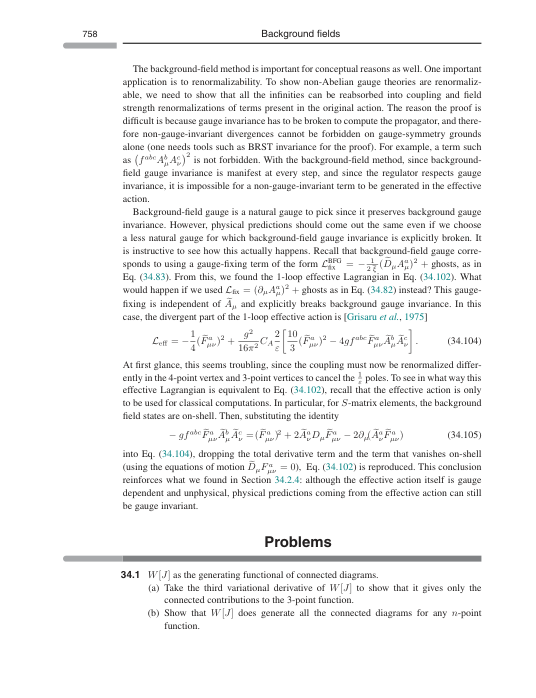
\includegraphics{./figs/34_Background_fields_page_778.png}

---

